\documentclass[../_main/handlingar.tex]{subfiles}

\begin{document}
\proposition{Renovering och ombyggnad av HK och Blådörren}

Så som det ser ut idag används inte större delar av Blådörren, rummet används framförallt till att hänga kläder och värma mat under lunchen. Om man sen kollar på HK så används detta rummet flitigt men eftersom rummet är så litet som det är kan max 2-3 personer sitta och arbeta samtdigt. Detta försvårar arbetet för alla som ska utföra admistrativt arbete för Sektionen men framförallt för styrelsen, ett större rum hade gjort att fler personer kunnat jobba parallellt. Vi skulle därför vilja ändra proportionerna på rummen till ungefär det motsatta från nuläget samt renovera upp rummen och införskaffa nya inventarier. Bilden nedan är ett förslag på hur rummen kan utformas men inte begränsat till det.

\begin{center}
    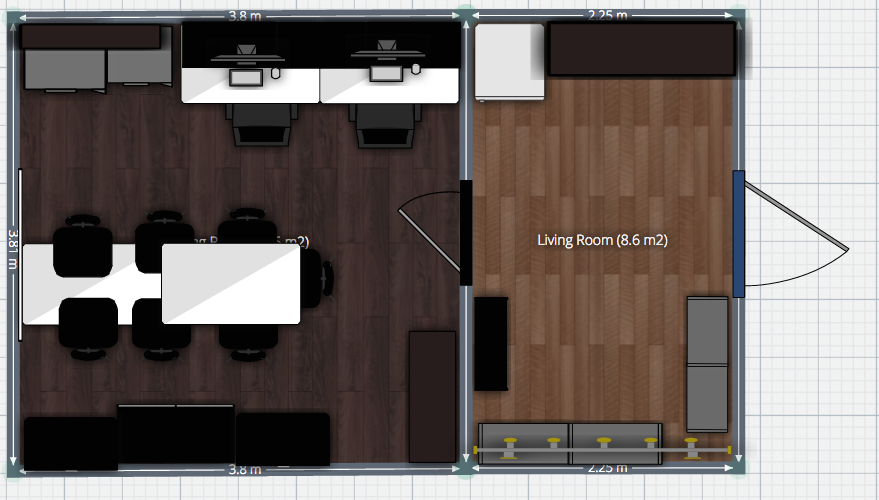
\includegraphics[width=13cm]{hkbla.png}
\end{center}

Därför yrkar vi på
\begin{attsatser}
    \att ändra om proportionerna på rummen så blådörren motsvarar 1/3 och HK motsvarar 2/3 av hela rummet.
    \att de som arbetar ska tackas med mat när det jobbar samt matbiljetter 40kr/st som som kan lösas in under hösten mot mat eller dylikt i LED eller klägg på gille.
    \att en budget på 30000kr avsätts till projektet. Budgeten ska täcka renoverings/ombyggnadskostnaderna, inköpskostnader av möblemang samt mat/tack-kostnader.
    \att kostnaden belastar utrustningsfonden.
\end{attsatser}

\begin{signatures}{2}
    \ist
    \signature{Anders Nilsson}{Förvaltningschef}
    \signature{\ordf}{Ordförande}
\end{signatures}

\end{document}
